
\subsection{Infrastruktur und Code-Entwicklung}


\subsubsection{Infrastruktur}

Die für dieses Projekt eingesetzte Infrastruktur setzt auf verschiedene Komponenten, deren Zusammenspiel hier in einer vereinfachten Darstellung zu sehen ist und im Folgenden näher beschrieben wird: 

\begin{figure}[H]
    \centering
    \label{fig:henning-dia-git-dev-server}
    \caption{Konzept: Entwicklung, Codeverteilung, Produktivnahme}
    \fbox{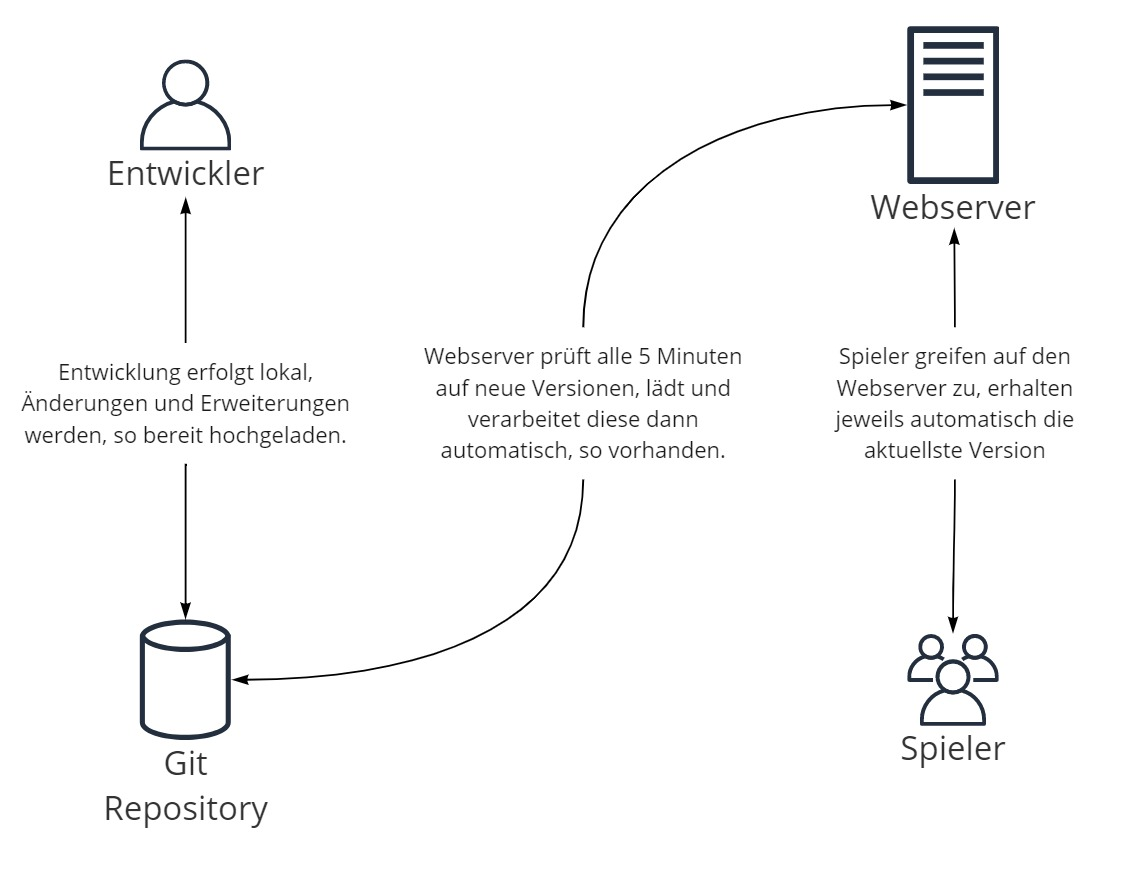
\includegraphics[width=0.8\textwidth]{henning-dia-git-dev-server}}
\end{figure}


Die Dienste selbst laufen auf einem für dieses Projekt bei der \textbf{HostEurope GmbH}\footnote{Siehe \url{https://www.hosteurope.de/Server/Virtual-Server/}.} angemieten, virtuellem Server. Das Produkt nennt sich \enquote{Virtual Server 10.0} und verfügt in der geringsten Austattung über 1 vCPU, 2 GB RAM sowie 40 GB SSD-Speicher. Auf dem Server läuft Debian 11. Der Server hat außerdem eine feste IP-Adresse. Einrichtungskosten gab es keine. Der Vertrag ist montalich kündbar. Der Mietpreis beträgt 5,99 EUR incl. MwSt. monatlich.

Weiter wurde bei \textbf{INWX GmbH}\footnote{Siehe \url{https://www.inwx.de/de/de-domain}.} zu dem Server auch eine Domain gekauft sowie entsprechende Namensservereinträge hinterlegt, die den Betrieb eines Traefik-Proxys mit Subdomains zu Domain erlauben. Auch hier gab es keine Einrichtungskosten. Der Preis für die Domain beträgt pro 5,97 EUR incl. MwSt. pro Jahr. 


Abseites der vorgenannten Hardware, stellt das gemeinsame \textbf{Git-Repository auf Github}\footnote{Siehe \url{https://github.com/tstsrv-de/rpg/}.} einen zentralen Punkt der Infrastruktur dar. In diesem Repository liegen alle Elemente des Projektes: Code, Skripte und Dokumentation.

Die Funktionen des Repositorys sind folgende: \begin{itemize}
    \item Entwickler übermitteln neue Inhalte in das Repository (push).
    \item Entwickler erhalten den stets aktuellen Entwicklungsstand aus dem Repository (pull, fetch).
    \item Der Server lädt neue Inhalte aus dem Repository automatisch und aktualisiert die Dienste.
    \item Alle Beteiligten und auch Dritte können über das Repository die Entwicklung nachvollziehen. 
\end{itemize}


Für den Update-Prozess des Servers und der Dienste wurde ein Cron-Skript erstellt, dass laufend prüft ob neue Commits im Repository vorhanden sind (siehe \textbf{Codelisting 1} unten, Zeile 5). Wenn ja, wird der Django-Webserver gestoppt (Zeile 7), die neuen Inhalte heruntergeladen, verarbeitet und der Django-Webserver im Anschluss wieder gestartet (Zeile 15). 

\textbf{Codelisting 1: \enquote{rpg/server-update-cron.sh}, gekürzt um Logging:}
\begin{lstlisting}[language=bash]
#!/bin/bash
cd /home/rjhadmin/tstsrv/
now=$(date "+%F %H:%M:%S")
git -C /home/rjhadmin/tstsrv/ fetch origin 
if  [ `git -C /home/rjhadmin/tstsrv/ rev-list HEAD...origin/main --count` != 0 ] 
then
    docker-compose --project-directory /home/rjhadmin/tstsrv/ stop rpg  
    git -C /home/rjhadmin/tstsrv/ reset --hard origin/main  
    git -C /home/rjhadmin/tstsrv/ fetch
    git -C /home/rjhadmin/tstsrv/ pull 
    chmod +x /home/rjhadmin/tstsrv/*.sh 
    docker-compose --project-directory /home/rjhadmin/tstsrv/ run rpg python rpg/manage.py makemigrations 
    docker-compose --project-directory /home/rjhadmin/tstsrv/ run rpg python rpg/manage.py migrate 
    docker-compose --project-directory /home/rjhadmin/tstsrv/ run rpg python rpg/manage.py loaddata db_sample_data.json 
    docker-compose --project-directory /home/rjhadmin/tstsrv/ start rpg 
\end{lstlisting}



Ein weiterer wesentlicher Punkt der Software-Infrastruktur sind die \textbf{Docker-Container} für den Django-Server, die Datenbank und den Reverse-Proxy. Hier stehen für die lokale Entwicklung \enquote{docker-compose}-Skripte für Windows und auch unixartige Systeme wie Linux und MacOS zur Verfügung. Ebenso für den Betrieb des Servers. Details zur Einrichtung und Nutzung wurden in der \textbf{Readme Repositorys}\footnote{Siehe \url{https://github.com/tstsrv-de/rpg/blob/main/README.md}.} hinterlegt. 


Der Traefik-Proxy wurde so eingerichtet, dass Anfragen auf den Ports HTTP 80 und HTTPS 443 angenommen werden. Anfragen an HTTP 80, werden automatisch umgeleitet an HTTPS 443. Die notwendigen Zertrifikate für die Subdomains werden vollautomatisch vom Traefik-Proxy über \textit{Letsencrypt} angefordert und verwaltet. Als Grundlage für die Konfiguration diente eine Vorlage von Igor Bubelov\footnote{Siehe Github-Repository dazu \url{https://github.com/bubelov/traefik-letsencrypt-compose}.} die entsprechend um die Funktionen für den Django-Webserver und die Datenbank erweitert wurden.

Die hier entwickelte Konfiguration erwies sich als so verlässlich, dass auch ein anderes Projektteam (\textbf{Deskshare\footnote{Siehe \url{https://github.com/tstsrv-de/deskshare} bzw. \url{https://deskshare.tstsrv.de/}.}}) aus unserem Studiengang, ihre Dienste auf unserer Hardware unter einer eigenen Subdomian betreiben konnte. Die Anbindung an den Traefik-Proxy war möglich, auch die SSL-Zertrifikate wurden vollautomatisch erstelt. Weiter konnte auch das Update-Konzepts mittels Cron-Dienst und Github-Repository übernommen werden, so dass das andere Projektteam eigenständig entwickeln konnte. 


Die Ressourcen des Servers reichen hier für beide Projekte, auch in der Phase vor Abgabe der Arbeiten, aus: 

\begin{figure}[H]
    \centering
    \label{fig:henning-server-auslastung}
    \caption{Bildschirmfoto: Server Auslastung}
    \fbox{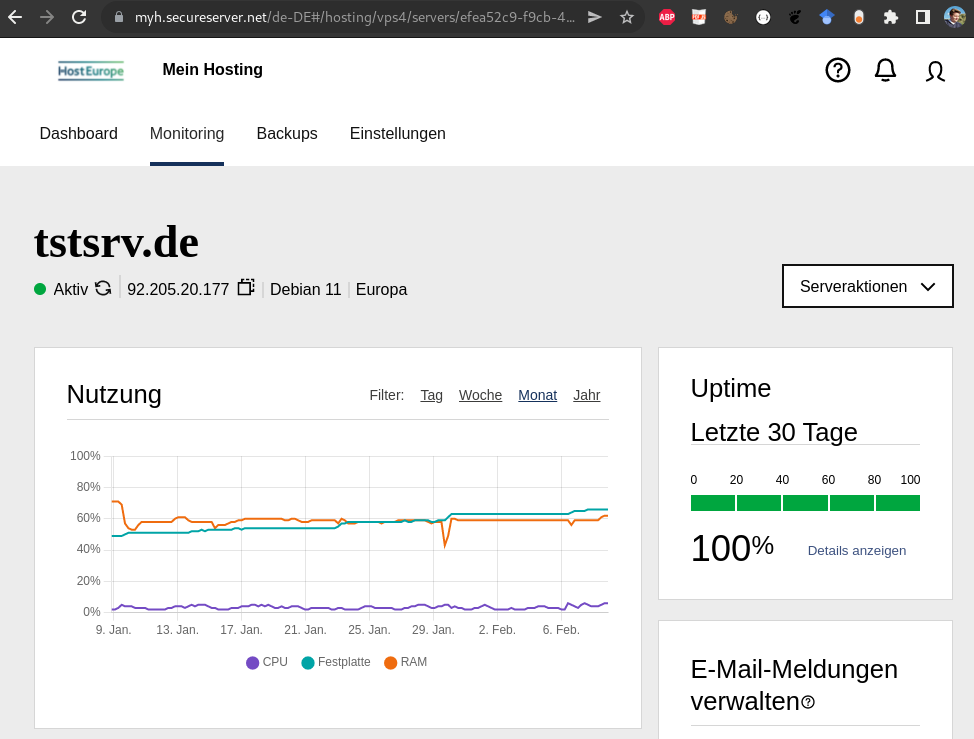
\includegraphics[width=0.8\textwidth]{server-auslastung.png}}
\end{figure}






\subsubsection{Initialisierung der Django-Anwendung}

Nach dem Aufbau der grundsätzlichen Funktionen des Servers (Update-Systemdienste und Cron-Skripte), wurde die Django-Anwendung initialisiert. Der Ablauf orientierte sich hier an den in den Vorlesungen gewonnenen Erkenntnissen und wurde im Anhang (siehe Anhang \ref{django-init}) stichpunktartig festgehalten. 

Im Anschluss daran wurden dann zuerst grundlegende Funktionen für die Benutzer-Regeistrierung am System hinzugefügt. Das geschah insbesondere unter Nutzung von zwei Anleitungen\footnote{Siehe  \url{https://www.nintyzeros.com/2020/06/login-register-user\%20page-in\%20django.html} und \url{https://docs.djangoproject.com/en/3.2/topics/auth/default/\#built-in-auth-forms}.}.


Da das Projekt selbst die Entwicklung eines Spiels umfasste, wurde hier bewusst auf die Implementation von allen ansonsten mit einer Benutzerverwaltung im Zusammenhang stehenden Funktionen verzichtet. Es ist somit \textbf{nicht möglich}, seinen Benutzer z.B. zu löschen oder \textbf{ein vergessenes Passwort} zu erneuern. Unser Fokus lag hier, den Anforderungen entsprechend, auf der Entwicklung der Hauptanwendung. 

Es wird hier in dieser Dokumentation auch nicht weiter auf die implementierte Benutzerverwaltung eingegangen, da es sich um weithin bekannte Standart-Features von Django handelt.

Mit Abschluss der Einrichtung der Django-Anwendung, liegt ein mit den bekannten Funktionen (wie Datenbankmodelle, Benutzerverwaltung, DB-Migrationen, ...) nutzbarer Django-Webserver vor. 
Für die Entwickler und die Entwicklung selbst ist die direkte Interaktion mit dem Django-Webserver nicht mehr notwendig. Die entwickelten Skripte starten den Webserver mit allen notwendigen Paramentern selbstständig und führen vorher auch notwendige Schritte wie \enquote{makemigrations, migrate oder loaddata} automatisch aus. Beispielhaft hier ein Auszug aus dem Skript für den Start der lokalen Entwicklungsumgebung unter unixartigen Betriebssystemen\footnote{Siehe \url{https://github.com/tstsrv-de/rpg/blob/main/local-dev-start.sh}.}: 

\begin{lstlisting}[language=bash]
#!/bin/bash
docker-compose -f local-dev-docker-compose.yml up -d
docker-compose -f local-dev-docker-compose.yml exec rpg python rpg/manage.py makemigrations
docker-compose -f local-dev-docker-compose.yml exec rpg python rpg/manage.py migrate
docker-compose -f local-dev-docker-compose.yml exec rpg python rpg/manage.py loaddata db_sample_data.json
docker-compose -f local-dev-docker-compose.yml stop
docker-compose -f local-dev-docker-compose.yml up 
\end{lstlisting}


\subsubsection{Datenbankmodell}

Aus den ersten Gesprächen und Austausch zum Projekt und den später formulierten Anforderungen wurden erste Konzepte und Ideen zu Papier gebracht. Dabei wurden auch erste Zeichnungen zu einem möglichen Datenbankmodell erstellt. In bzw. zu den späteren Projektbesprechungen wurden konkretere Zeichnungen erstellt. 

\begin{figure}[H]
    \centering
    \label{fig:henning-entwurf-datenbankmodell}
    \caption{Datenbankmodell Entwurfsprozess}
    \subfloat[Entwurfszeichnung vom 23.11.2021]{\fbox{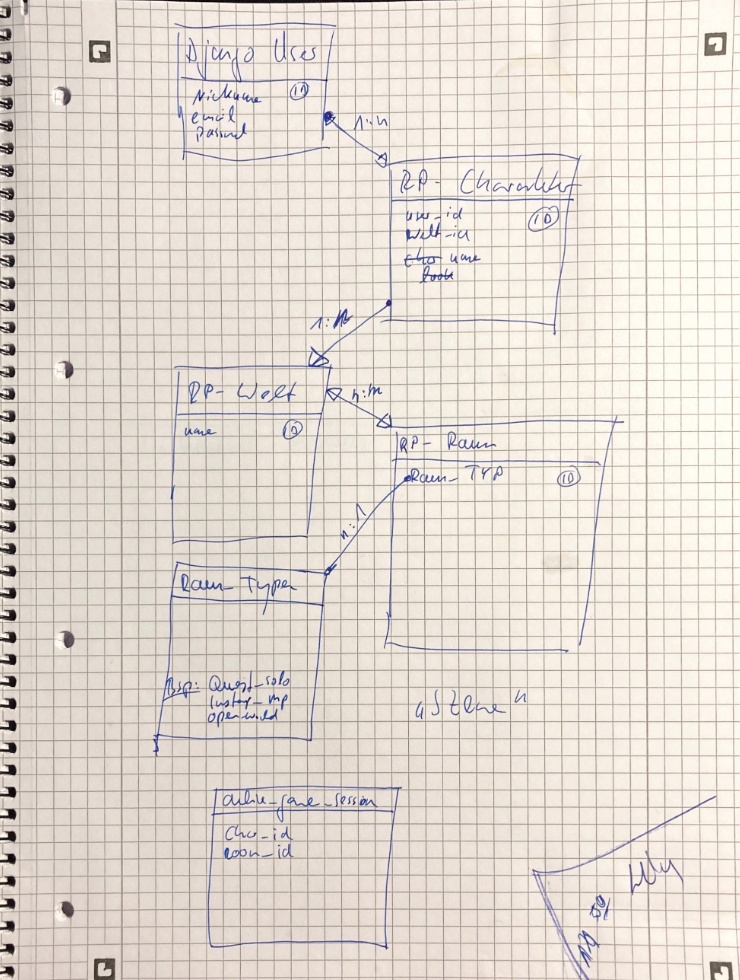
\includegraphics[width=0.5\linewidth]{2021-11-23-erstes-db-konzept}}}
    \subfloat[Weiterentwickelter Entwurf (05.12.2021)]{\fbox{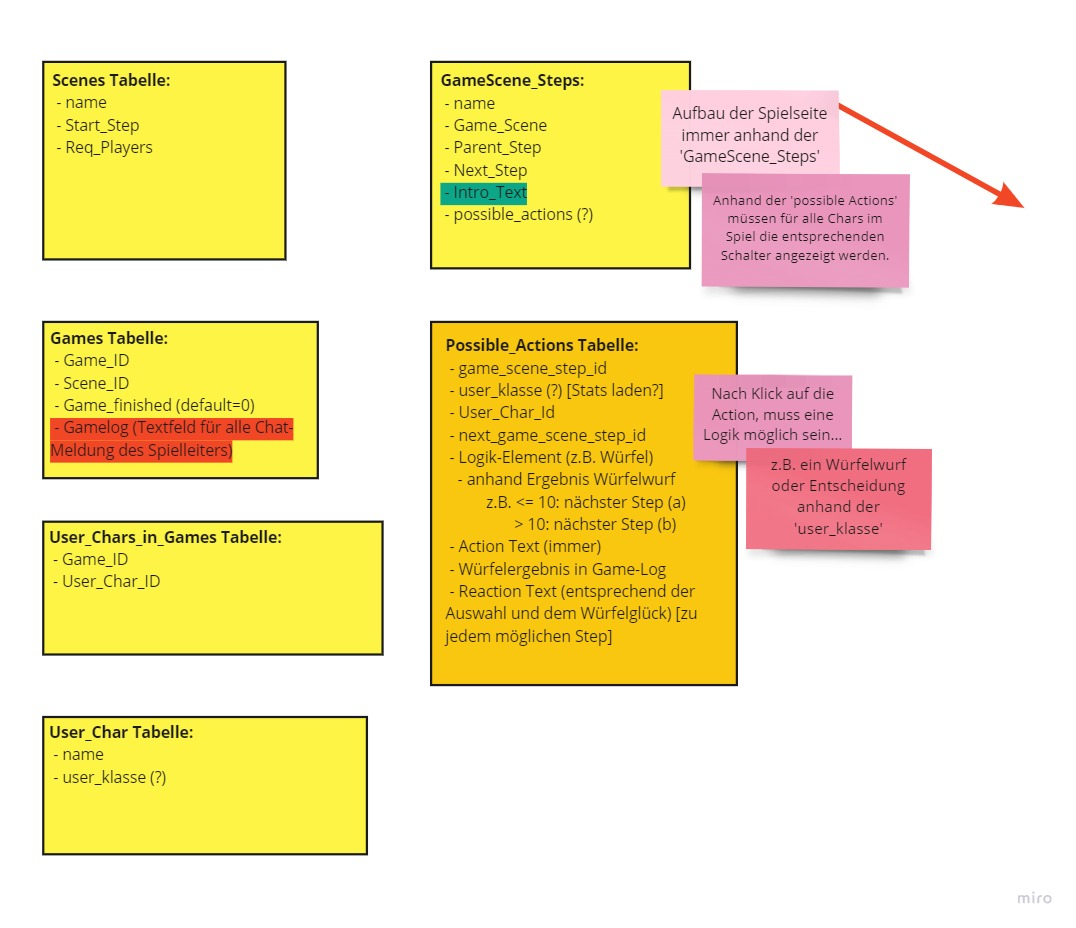
\includegraphics[width=0.5\linewidth]{2021-12-05-Projketbesprechung-Miro-c}}}
\end{figure}

Fortsetzung auf der Folgeseite. 

\newpage

Hier eine Darstellung des Datenbankmodells als Diagramm sowie anschließend die ausführliche Beschreibung jeweils mit Stand vom 10.02.2022. 

\begin{figure}[H]
    \centering
    \label{fig:henning-datenbankmodell-final}
    \caption{Datenbankmodell final (Stand 10.02.2022)}
    \fbox{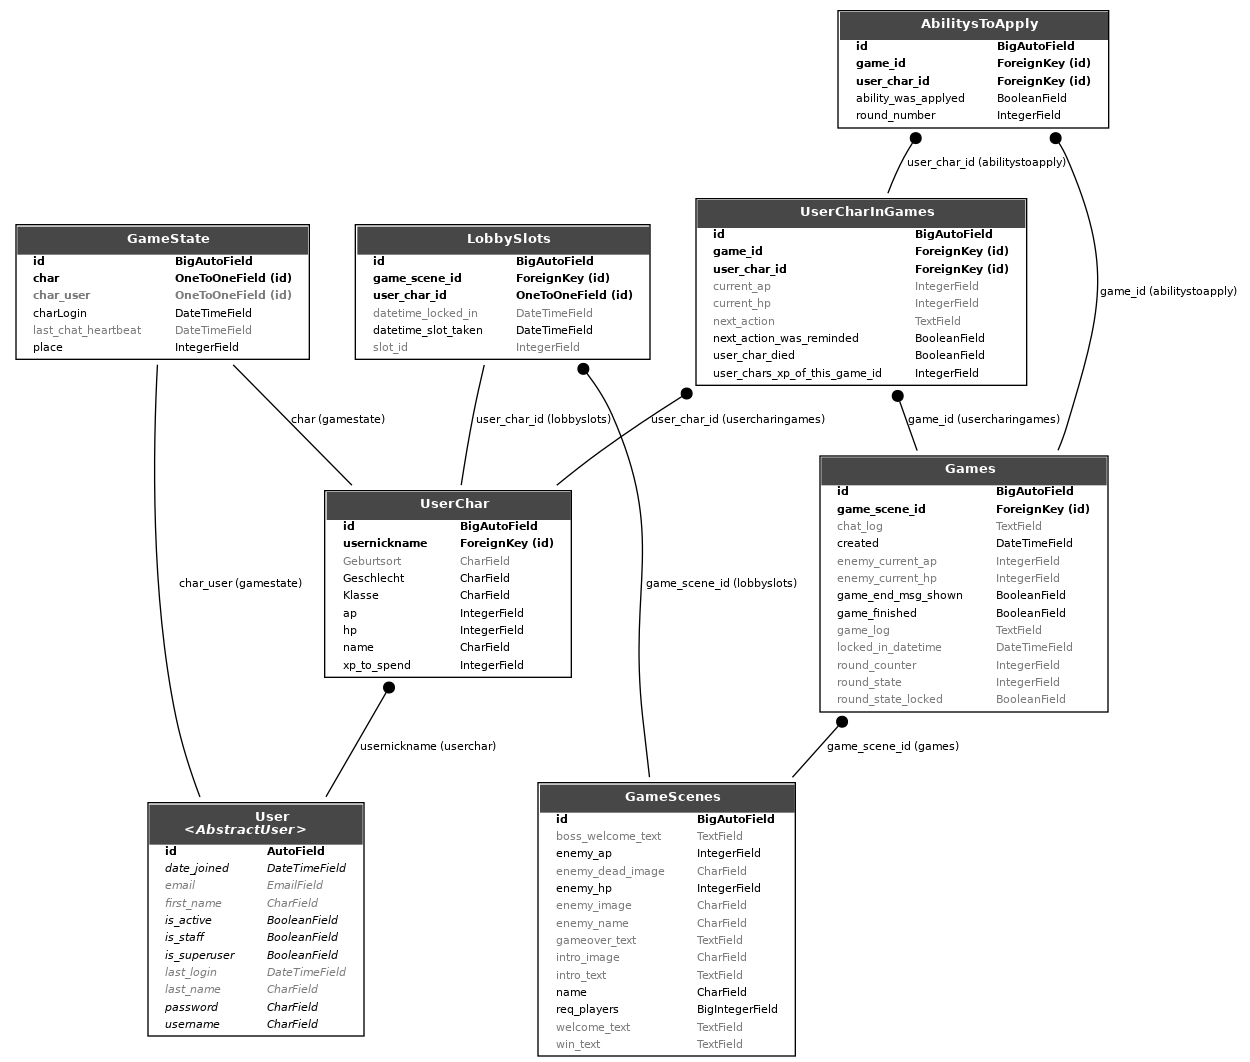
\includegraphics[width=0.8\textwidth]{db-modell-final.png}}
\end{figure}


Der Aufbau der des Datenbankmodells beginnt logisch mit der \textbf{Benutzertabelle}, sowie den anderen von Django systemseitig erstellten Tabellen, auf die hier nicht weiter eingegangen wird.

Auf die Benutzertabelle setzt eine \textbf{Tabelle für Charaktere} (\textit{UserChar}) auf. Darin enthalten und jeweils einem Benutzer zugeordnet, sind alle Daten zu den Spielercharakteren. Neben dem Namen und der Klasse sind in der Tabelle auch veränderliche Attribute wie die Angriffspunkte und Lebenspunkte sowie noch zu verteilende Erfahrungspunkte abgespeichert. 

Bei der Erstellung eines neuen Charakters werden die Start- bzw. Standartwerte für Lebens- und Angriffspunkte aus einer besonderen \textbf{Konfigurationstabelle} (\textit{myrpgconfig}) abgerufen und für die Erstellung des neuen Charakters, entsprechend der ausgewählten Klasse, abgespeichert. In diese Konfigurationstabelle wurden weiter auch \textbf{alle Konstanten}, die im Laufe der Entwicklung Einzug in den Programmcode gehalten haben transportiert. Dies umfasst tatsächlich komplett alle Konstanten. Beispielhaft genannt seien hier z.B. der Faktor für die Berechnung von Erfahrungspunkten aus dem verursachten Schaden, der Minimal- und Maximalfaktor bei der Berechnung des bei einem Angriff entstandenen Schaden aus den Angriffspunkten heraus sowie auch die Laufzeiten in Rundenzahl sowie die Stärke der Fähigkeiten der einzelnen Klassen. 

Das erlaubt es die gesamte Konfiguration des Projektes und ebenso auch das Balancing über die Administrationsoberfläche von Django unkompliziert zu verändern und zu pflegen. Die Konfigurationstabelle umfasst 21 Einstellungen. Zu jeder Einstellung sind in der Datenbank selbst auch entsprechende Erklärungen zur genauen Verwendung und Nutzung hinterlegt. Auch ist es möglich \textbf{verschiedene Datentypen in der Konfigurationstabelle} abzuspeichern und abzurufen. Folgende Hilfsfunktion wurde dazu in der Datei \enquote{rpg\_tools.py}\footnote{Siehe \url{https://github.com/tstsrv-de/rpg/blob/main/rpg/rjh_rpg/rpg_tools.py\#L63-L80}.} erstellt: 

\begin{lstlisting}[language=python]
def rpg_get_config(config_to_get):

    try: 
        config_type = MyRpgConfig.objects.get(name=config_to_get).type
    
        if config_type == "int":
            return int(MyRpgConfig.objects.get(name=config_to_get).value)

        elif config_type == "str":
            return str(MyRpgConfig.objects.get(name=config_to_get).value)

        elif config_type == "float":
            return float(MyRpgConfig.objects.get(name=config_to_get).value)
    
    (...)
\end{lstlisting}


Neben der Benutzer-, Charakter- und der Konfigurationstabelle gibt es eine ganze Menge an Tabellen für das Spiel selbst. Zentral ist dabei die \textbf{Grundtabelle der Level} (\textit{GameScenes}): Diese ist als Bauplan der Level zu verstehen. Enthalten sind alle notwendigen Informationen um ein neues Spiel in einem der Level starten zu können: Der Name des Gegeners, die Texte und Werte des Gegners. Aber auch die Anzahl der für diesen Level notwendigen Spieler. Ebenso sind alle Texte zum Level (Intro, Gewinn- und Gameover-Nachricht etc.) darin enthalten. 

In der \textbf{Hilfstabelle für den Spieler-Staus} (\textit{GameState}) wird jeweils der aktuelle Standort eines Spielers hinterlegt. Mit Standort ist dabei die aktuell aufgerufene Seite des Spieles gemeint. Es kann darüber nachvollzogen werden ob der Spieler sich gerade auf der Weltkarte befindet oder in einer der Level-Lobbys. Auch wird darin ein Zeitpunkt des letzten Datenpaketes aus dem Chat hinterlegt. Darüber ist es möglich, Spieler nach Ablauf einer gewissen Zeit (Sekunden), automatisch aus dem Chat zu entfernen. 

Innerhalb der Level-Lobby können über die \textbf{Hilfstabelle für die Level-Lobbys} (\textit{LobbySlots}) die bereits belegten Plätze für ein Spiel nachgehalten werden. Die Spieler belegen in der Lobby mit einem Klick einen verfügbaren Platz. Sind dann alle Plätze des Levels belegt, wird nach Ablauf eines Countdowns \textbf{ein neues Spiel gestartet}.

Mit Spielstart wird in der \textbf{Spieltabelle} (\textit{Games}) ein neues Spiel angelegt. Dieses Spiel darin trägt eine Verknüpfung zum Bauplan (Grundtabelle der Level: \textit{GameScenes}), ein Game-Log in dem alle Texte des Spiels gespeichert werden, die aktuellen Lebens- und Angriffspunkte des Gegeners sowie auch alle \textbf{Informationen zum Rundenstatus} des Spiels.

Gleichzeitig mit der Anlage des Spiels selbst, werden in der \textbf{Hilfstabelle für die Spieler- und Spiel-Zurodnung} (\textit{UserCharInGames}) für jeden für das Spiel angemeldeten Spieler ein entsprechender Eintrag erzeugt. Während des Spiels werden darin alle Werte des Spieler hinterlegt. Auch ob der Spieler in diesem Spiel bereits verstorben ist, wird darin gespeichert. 

Letzte mit dem Spielablauf im Zusammenhang stehende Tabelle ist eine \textbf{Spezialtabelle für die aktivierten Fähigkeiten der Spieler} (\textit{AbilitysToApply}). Darin wird immer wenn in einem Spiel ein Spieler seine Fähigkeit aktiviert, alle Informationen abgespeichert die für die spätere Wirksamkeit notwendig sind. Entscheidet sich z.B. der Priester in Runde 3 seine Fähigkeit anzuwenden (und wirkt diese über 4 Runden), werden in der Tablle entsprechende Einträge für Runde 4, 5, 6 und 7 mit Bezug auf den Priester und die Heilung hinterlegt. Wendet die Runden- bzw. Spiellogik diese Fähigkeit an, wird ein entsprechndes Kennzeichen dazu in dem Datensatz gesetzt (\textit{ability\_was\_applyed = true}).





\subsubsection{Hervorzuhebende Code-Entwicklungen}


Neben Standard-Entwicklungen wie z.B. Registrierungs- und Loginfunktionen (die hier wie bereits klar gemacht, nicht weiter beschrieben werden sollen), wurden vor allem sehr spezifische Entwicklungen durchgeführt. Im nun folgenden Abschnitt werden insbesondere zwei Teile näher beschrieben: 

\begin{enumerate}
    \item Die Funktionsweise und Implementation der Websockets, sowie 
    \item die Rundenlogik im Spielverlauf.
\end{enumerate}



Zu den \textbf{Websockets} wurden im Kapitel \nameref{anforderungen} einige Grundlagen bereits erklärt. Bei der Entwicklung wurde hier als erster Programmteil nach den Basisfunktionen, eine Chat-Funktion über die Websockets implementiert. 


Dies vor allem unter Nutzung einer Anleitung\footnote{Siehe \url{https://github.com/veryacademy/YT-Django-Project-Chatroom-Getting-Started}.}, die eine Basis-Form der Chat-Funktionalität bereitstellte. Diese wurde schnell für die in diesem Projekt beachsichtigten Zwecke erweitert und angepasst:

In der nun vorliegenden Lösung öffnet sich beim \textbf{Besuch der Worldmap}, über das dargestellte Chatfenster eine Websocket-Verbindung. Diese bleibt als offene Verbindung bestehen und erlaubt es Nachrichten zwischen dem Server (Django) und dem Client (Browser) auszutauchen. Auf der Serverseite läuft dies innerhalb Djangos über ein Routing der Websockets in entsprechende Consumer-Funktionen. Auf Clientseite findet JavaScript Verwendung für das Versenden sowie Empfangen und Verarbeiten der Nachrichten über das Websocket-Protokoll. 

Innerhalb der \textbf{Level-Lobby-Seiten} wird jeweils auch eine entsprechende Websocket-Verbindung aufgebaut. Über die ID der Lobby, wird hier analog eine Websocket-Verbindung mit gleicher ID aufgebaut. Die Zuordnung des Aufrufs erfolgt hier innerhalb von Django über die in der \textit{settings.py} hinzugefügte App \textit{channels} sowie die Einstellungen zur ASGI-App \textbf{mit dem Routing-Ziel} zur enstpechdenen Auflösung des Websockets-Aufrufs über die \textit{routing.py} innerhalb der Django-App \textit{rjh\_rpg}:

\begin{lstlisting}[language=python]
websocket_urlpatterns = [
(...)
    re_path(r'ws/lobby-(?P<scene_id>\w+)/$', consumer_lobby.Consumer.as_asgi()),
    re_path(r'ws/game-(?P<game_id>\w+)/$', consumer_game.Consumer.as_asgi()),
]
\end{lstlisting}

Der Aufbau von Websocket-Verbindungen ist, wie man sieht, analog der aus Django bekannten \enquote{urls.py} geregelt. Von \textbf{Client-Seite} aus wird hier eine bestimmte URL aufgerufen und damit die Websocket-Verbindung aufgebaut. Über das Objekt dieser aktiven Verbindung können dann Nachrichten (hier als JSON-String) übermittelt werden, beispielhaft und stark vereinfacht wie folgt: 


\begin{lstlisting}[language=JavaScript]
const chat_websocket = new WebSocket("wss://rpg.tstsrv.de/worldmap-chat/");
chat_websocket.send(JSON.stringify({ user: user_id, message: message, }));
\end{lstlisting}



Als nächsten Entwicklungsschritt wurden hier dann die \textbf{veränderlichen Webseiteninhalte über Websockets} transportiert - Ähnlich AJAX bzw. einem Framework mit Nutzung einer API als Backend. In dem Anwendungsfall unseres Spiels findet hier die Verarbeitung vor allem in dem Websockets-\textit{Consumer} für das Spiel statt: der \textbf{consumer\_game.py}.

Darin werden vom Client erhaltene Nachrichten verarbeitet. Diese Nachrichten können z.B. das Klicken eines der Buttons sein (Angriff, Fähigkeit, Aussetzen) oder auch ein laufend übersendetes Lebenszeichen, ein \textit{Heartbeat}. Dieser teilt dem Server mit, dass der jeweilige Spieler noch im Spiel ist und die Webseite offen hat, die Websocket-Verbindung also noch Bestand hat. Stark vereinfacht und gekürzt stellt sich das im Programmcode wie folgt dar: 

\begin{lstlisting}[language=python]
class Consumer(AsyncWebsocketConsumer):
 
    # Verbindungsaufbau
    async def connect(self):
        self.game_id = self.scope['url_route']['kwargs']['game_id']
        self.msg_group_name = 'game-%s' % self.game_id

        await self.channel_layer.group_add(
            self.msg_group_name,
            self.channel_name
        )

        await self.accept()

    # Neue Nachricht alle Empfänger der Websockets-Gruppe (hier Spieler des Spiels) senden
    async def msg_group_send_game_log_update(self, event):
        game_log_content = await db_get_game_log(self.game_id)
        
        if game_log_content == self.last_game_log_content:
            # skip sending if no change since last message
            pass
        else:
            await self.send(text_data=json.dumps({ 
                'game_msg_type': 'game_log_update',
                'game_websocket_content': str(game_log_content),
            }))
            self.last_game_log_content = game_log_content

    # Empfang und Verarbeitung erhaltener Nachrichten
    async def receive(self, text_data):
        text_data_json = json.loads(text_data)
        message = text_data_json['msg']

        if message == 'alive':
            round_state = await db_get_round_state(self.game_id)

            # Hier finden sich rund 300 Zeilen Code der die Spiel- und Rundenlogik abbildet
                
            # Mit Ende der Verarbeitung werden neue Informationen an die Spieler des Spiels übersandt

            await self.channel_layer.group_send(self.msg_group_name, { 
                                'type': 'msg_group_send_game_log_update', })
\end{lstlisting}
    

Man sieht, dass die Spielelogik im Wesentlichen durch den Erhalt von Nachrichten fortgeführt bzw. -geschrieben wird.  Das Spiel durchläuft dabei Runden, die in Rundenstufen unterteilt sind. Innerhalb dieser Rundenstufen werden verschiedene Aktionen oder Prüfungen durchgeführt. Auch werden in einer Rundenstufe z.B. die Aktionen der Spieler eingesammelt. Das bedeutet, dass das Spiel solange in dieser Rundenstufe (Aktionen einsammeln) verbleibt, bis jeder Spieler eine nächste Aktion ausgewählt hat. 

In der Projektbesprechung vom 11.12.2021 wurde ein Rundenablauf erarbeitet, der übersetzt als Pseudo-Code Grundlage für die Programmierung wurde: 

\begin{enumerate}
    \item Aktion von Gegner ausführen (Schaden) [100]
    \item Prüfen ob User-Char tod ist (HP < 1 = Dead-Flag: True) [200]
    \item Prüfen wie viele User-Chars noch leben (n < 1 = Gameover-Flag: True, break-Gameloop-Schleife) [300]
    \item Aktionen der User-Chars aufnehmen (Entscheidung für nächste Aktion von jedem Spieler annehmen + wegspeichern) [400]
    \item Alle Aktionen der User-Chars ausführen (Aktionen laden und ausführen: Schaden, Aktion, Passen) [500]
    \item Nach jedem Spieler, prüfen ob Gegner besiegt wurde (HP < 1 = Win-Flag: True, break-Gameloop-Schleife) [immernoch 500]
    \item Rundencounter +1 [600]
    \item Gameloop-Schleife nächster Durchlauf [700, zurück zu 100]...
\end{enumerate}

Mit Abschluss der Programmierung ergab sich ein etwas detailierterer Rundenablauf, der im Code dann wie folgt fixiert wurde und hier dokumentiert ist: 


\begin{lstlisting}
# all round states in game-loop:
  0 inital for new games
 50 apply effects of used abilitys
100 enemy makes damage
200 check user-chars with less than 0 hp, mark them as dead
300 check if any user-chars are alive, if not end game with gameover-flag 990
400 collect and save the next actions from all alive user-chars, proceed only every user-char has a next action set
500 run the collected actions (make damage, use ability, pass turn), check after each user-char if enemy is alive, if not end game with win-flag 995
600 increase round\_counter + 1
700 reset round\_state and loop to 50

# round-states without looping anymore:
990 gaveover / game lost
995 game is won
999 show link to exit
\end{lstlisting}

Tests ergaben Probleme beim Spiel mit mehreren Spielern. Die Rundenlogik wurde gleichzeitig vorangetrieben. Dadurch wurden manche Aktionen und Rundenschritte mehrfach ausgeführt. Ein Versuch das Problem mit einem Token (ähnlich einem Semaphor) zu lösen, brachte leider keinen abschließenden Erfolg. Der Einzelspieler aber funktionierte fehlerfrei. 

Als Workaround für oben genanntes Problem im Mehrspieler wurde eingestellt, dass immer nur der erste Spieler eines Spiels die Rundenlogik vorantreibt. Das ist etwas fehleranfälliger als eine korrekte Token-Lösung, wird für das Projekt hier aber vorerst ausreichend sein (Commit \url{https://git.io/Jy1su}).

Die Hauptentwicklungsphase endete mit einer Spielseite, die sich noch farbenfroh darstellte: 

\begin{figure}[H]
    \centering
    \caption{Bildschirmfoto der Spieleseite zum Entwicklungsstand per 29.12.2021}
    \label{fig:2021-12-29-Bildschirmfoto-Entwicklungsstand-Runden-Status-400.png}
    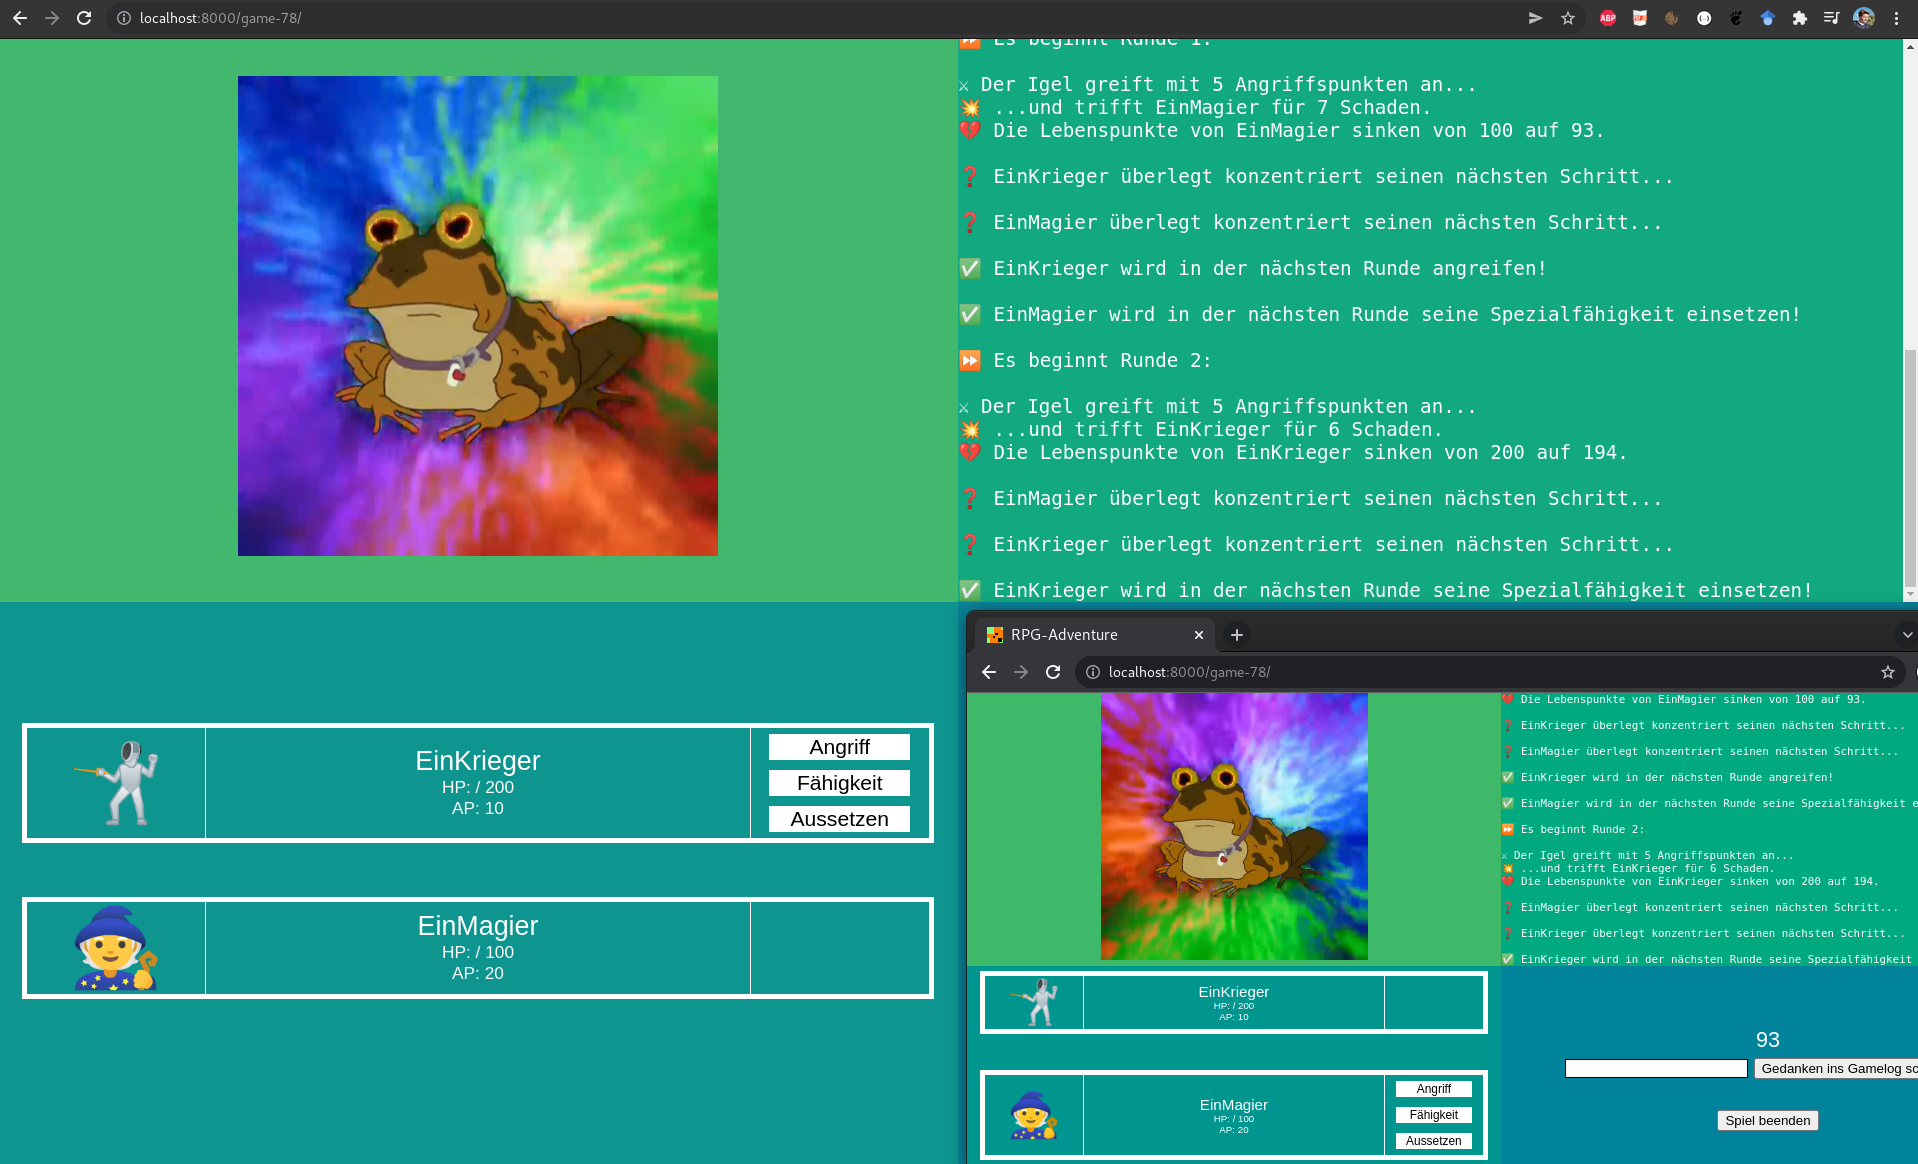
\includegraphics[width=0.7\textwidth]{2021-12-29-Bildschirmfoto-Entwicklungsstand-Runden-Status-400.png}
\end{figure}
    
